\chapter{Double Chooz: First Hints of $\theta_{13}$}
\label{chap:Double Chooz}
\section{The State of the PMNS Matrix}
In the time since the confirmation of neutrino oscillations by SNO, a great deal of experimental work has been performed to determine the values of the terms of the PMNS matrix. The values can be referenced by their position within the matrix or by the most common method of detection. For example, the mixing angle $\theta_{12}$ and associated mass difference $\Delta m_{12}^2$ is termed ``solar"  as solar electron neutrinos are source particles for the experiments. A long baseline is required for maximal oscillation between mass state 1 and 3. Similarly, the mixing angle  $\theta_{23}$ is the atmospheric mixing angle, due to the use of atmospheric muon neutrinos as a source particle and the mixing angle $\theta_{13}$ is the reactor neutrino mixing angle (though $\theta_{12}$ is sometimes also termed a reactor neutrino angle as well). 

The Chooz experiment was an early attempt to measure the reactor neutrino ($\theta_{13}$) mixing angle. Based outside of the Chooz nuclear power plant, it was not able to observe oscillation, but was able to set an upper on the value of the $\sin^2(2\theta_{13}) < .17$, assuming a large $\Delta m^2$ \cite{Chooz}. To improve upon the Chooz results, a new collaboration (Double Chooz) was formed, with a plan to quickly, cheaply, and accurately measure the mixing angle $\theta_{13}$, or at least reduce the upper bound significantly. 

Double Chooz would improve upon the Chooz bound in two primary ways. First, by introducing a second detector it is possible to normalize the reactor flux and eliminate uncertainties caused by reactor thermal power output. Second, Double Chooz would utilize improved technology and techniques to increase energy resolution and neutrino detection, allowing for improvement over the Chooz bound during the initial one-detector phase of operation.

\section{The Double Chooz Detectors}
 Double Chooz, like Chooz before it, is built near the Chooz nuclear power plant. The primary scientific apparatus of Double Chooz lies in two detectors: the Near and Far Detector. Figure \ref{DC_Picture} illustrates the near and far detectors, along with their relationship to the reactors. 
 \begin{figure}[h!]
  \caption{The near and far detectors \cite{DCWhitepaper} with their distances to the reactors.}
  \centering
    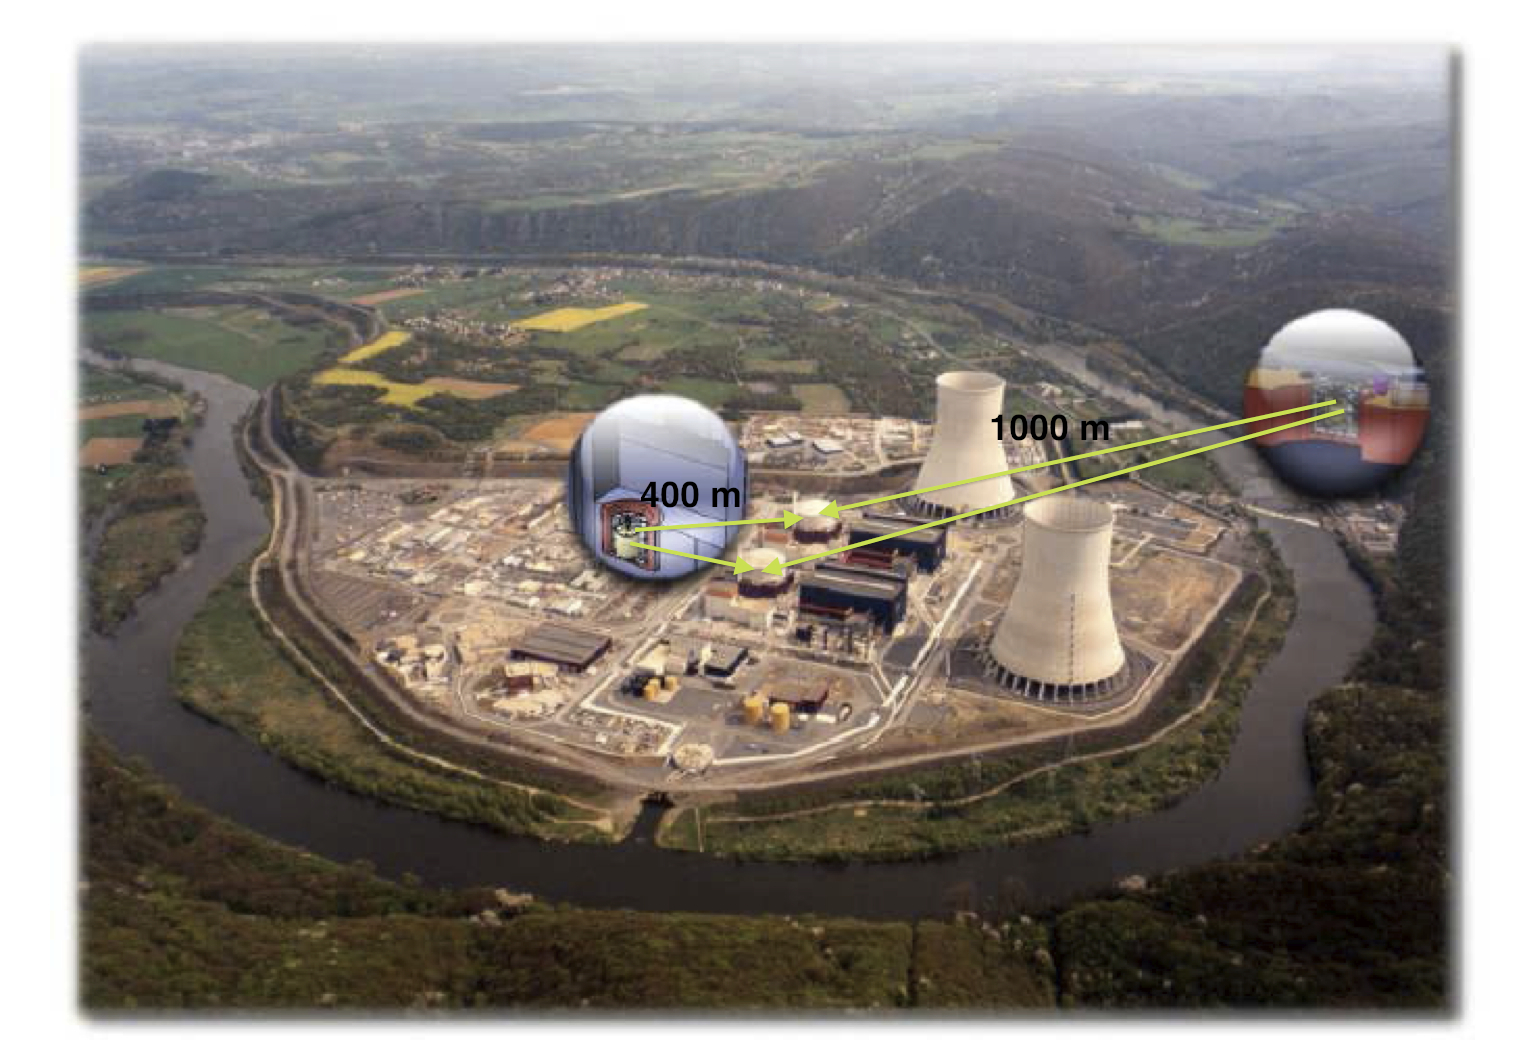
\includegraphics[width=\textwidth]{DC_Results/Chooz_Plant_Edit.jpg}
    \label{DC_Picture}
\end{figure}
 
The detectors consist of a series of co-centric cylinders, as can be seen in Fig. \ref{X_Section}. Beginning from the innermost, we have the neutrino target (NT). The NT is a sensitive region 115 cm in radius and 245.8 cm in height filled with gadolinium-loaded liquid scintillator, separated from other volumes by an acrylic vessel. Around the NT is the $\gamma$ catcher (GC), which is also filled with scintillator, but is not gadolinium-doped.  This GC is also surrounded by an acrylic vessel. Outside of the GC vessel is the buffer, which is loaded with mineral oil and is surrounded by a stainless steel enclosure. The buffer is designed to act as a non-sensitive region to help filter out background signals and is instrumented with photomultiplier tubes, or PMTs, designed to detect the signals originating in the NT. Finally, the outermost volume is the inner veto (IV), which is a scintillator-filled stainless steel vessel designed for vetoing muons and external radiation.



\begin{figure}
\caption{Side view of the Double Chooz Far Detector \cite{DC_2012}.}
\centering
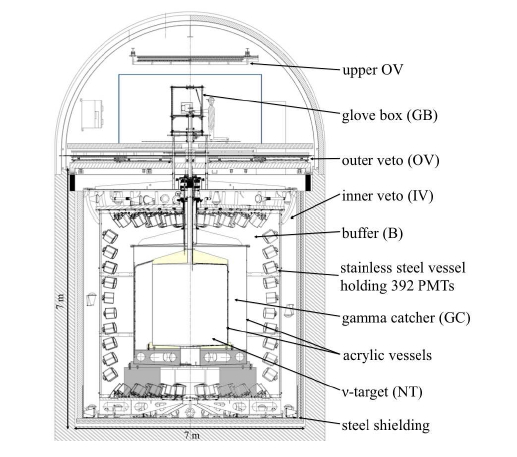
\includegraphics[width=.5 \textwidth]{DC_Results/Double_Chooz_Xsection.jpg}
\label{X_Section}
\end{figure}

\section{Experimental Setup}
The neutrino target (NT) is similar to the early neutrino experiments of Cowan \cite{Cowan}. It is filled with a mixture of dodecane and PXE (Phenyl-XylylethanE) in a 80:20 volume mixture ratio. The dodecane slightly reduces the light yield (78\% of pure PXE) of the scintillator \cite{DCWhitepaper}, but increases compatibility with the acrylic vessels.  This liquid mixture is doped with gadolinium, in the form of Gd-loaded carboxylic acid in a concentration of 1 g per liter of target scintillator.

The NT is the sensitive volume, in which $\bar{\nu_e}$ from the nearby reactors will interact via inverse beta decay: $\bar{\nu_e} + p \rightarrow n + e^{+}$. The vast majority of the kinetic energy of the incoming neutrino will be transferred to the positron. The positron will then rapidly annihilate with electrons in the target, producing a pair of annihilation $\gamma$'s. The gamma rays and the kinetic energy of the $e^{+}$ produce scintillation light, which is then detected by the 390 PMTs mounted on the inside of the buffer vessel. 

The neutron, meanwhile, will thermalize within 20.5 $\mu$s, then diffuse and be captured on the gadolinium with a capture time of approximately 30 $\mu$s, producing a shower of $\gamma$s with a total energy of 8 MeV. The neutron can capture on other elements in the target, most notably, hydrogen and carbon, but the neutron cross section for the gadolinium is much larger.  The basis for Double Chooz neutrino detection is to look for this double signal: prompt positron annihilation followed by a delayed Gd capture. While inverse beta decay can occur elsewhere in the detector, the other regions lack the gadolinium that produces the delayed event. 

With that said, there are a number of events that are either ``gained" or ``lost" because of neutron transport across the GC/NT boundary. The events that are gained are termed ``spill-in," while events that are lost are termed ``spill-out." To first order, the number of spill-in and spill-out events are identical, but closer examination of this effect is essential to a proper calculation of the sensitive volume of the experiment, and the proper calculation of $\theta_{13}$.  This task is best accomplished through the use of calibration systems, such as the Articulated Arm, detailed in Chp. \ref{chap:AA}.

As previously noted, the detection devices for Double Chooz are photomultiplier tubes (PMTs). Specifically, Hamamatsu R7081 10 inch PMTs with low-radiation glass are used for the buffer. The PMTs are supplied with high voltage to ensure a gain of $10^7$. The testing procedure used to assure this gain will be detailed in Sec. \ref{sec:PMT_Calibration}. The signal from these PMTs is sent to the data acquisition system (DAQ), which consists of three principle parts: the Front End, the FADC (Flash ADC), and the Trigger. A block diagram of the system can be seen in figure \ref{Block Diagram}

\begin{figure}
\caption{Double Chooz detector electronics  block diagram.}
\centering
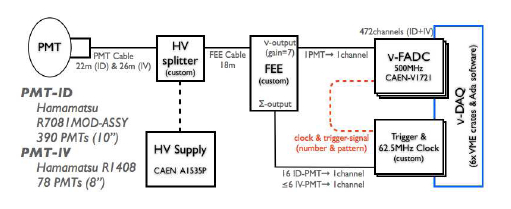
\includegraphics[width=.5\textwidth]{DC_Results/DC_Block_Diag.jpg}
\label{Block Diagram}
\end{figure}

The Front End is designed to optimize pulses: amplifying, clipping, and performing baseline restoration of input pulses, as well as filtering coherent noise, and delivering summed signals to the trigger. Pulses from the Front End are sent to the FADC for digitization. The total volume of data if all pulses would be retained would be very large, so a Trigger system is in place to act as a ``pre-filter" on signals. The Trigger works by comparing the summed pulses sent by the Front End to the input amplitude after the end of the pulse window. The signal difference required is 350 keV of deposited energy, which causes no trigger inefficiencies. The analysis threshold for neutrino signals is 0.7 MeV of deposited energy and the minimum deposited positron energy in a neutrino event is 1.02 MeV, far above the trigger threshold.  In addition to filtering out small signals, the trigger also acts as a high-pass filter, since very slow signals will not change substantially between the initial signal and the comparison after the pulse window. 

The final element of the DAQ is the FADC, which continuously writes to a buffer. The buffer can hold up to 1024 4-microsecond waveforms. When a trigger occurs, a waveform of 256 ns is recorded. The FADC saturates at signals $>$100 MeV, far in excess of the expected neutrino signal. The FADC baseline is stable to within an ADC count normally, however, after power-cycling, small ($<$ mV level) shifts in the baseline have been observed. The effect of these changes to the baseline could cause distortion in signals of less than 2 PEs, but steps were taken to minimize the effects of the baseline shifts. 

\subsection{Alternate Analysis Tool}
  Raw data from the buffer is in the form of 2 ns binned current from each PMT. This data is then run through the RecoPulse algorithm, which takes the raw data and chops it into a finite set of ``pulses," and correlates them into events, which correspond to a number of pulses with a similar start-time. This necessitates throwing out a large amount of empty data, which is to say, data in which there is either an insufficient amount of charge in a pulse, or the ``depth" (amplitude) of the pulse is below a certain threshold. The data with small or shallow signals is thrown out to try to reduce the amount of PMT noise. However, there is a risk of throwing out channels which have a small amount of charge, introducing energy- and position-based distortions into the reconstructed energy of an event. 
  
The risk primarily is because of the discrete photo-electron response of the PMTs. A PMT relies on the photoelectric effect,  producing an discrete number of electrons. These photo-electrons are then drawn through a series of stages, with the number of total electrons increasing at each stage. The entire process begins with an discrete number of electrons, resulting in a ``smallest" possible signal: the single photoelectron.

Despite the fact that there is a ``smallest" signal, not all ``smallest" signals are identical. For PMTs, there are two types of single photoelectron signals: exponential and Gaussian, depending on the PMT model. Gaussian-type responses produce single photoelectron signals which look roughly Gaussian, as the name suggests, while exponential-type responses are reasonably well-described by a decaying exponential. You can see an example of a Gaussian-type single photoelectron response (SER) in Fig. \ref{Gaussian SER}. 

\begin{figure}
\caption{Sample Gaussian single photoelectron response (SER) also showing the pedestal (brown).}
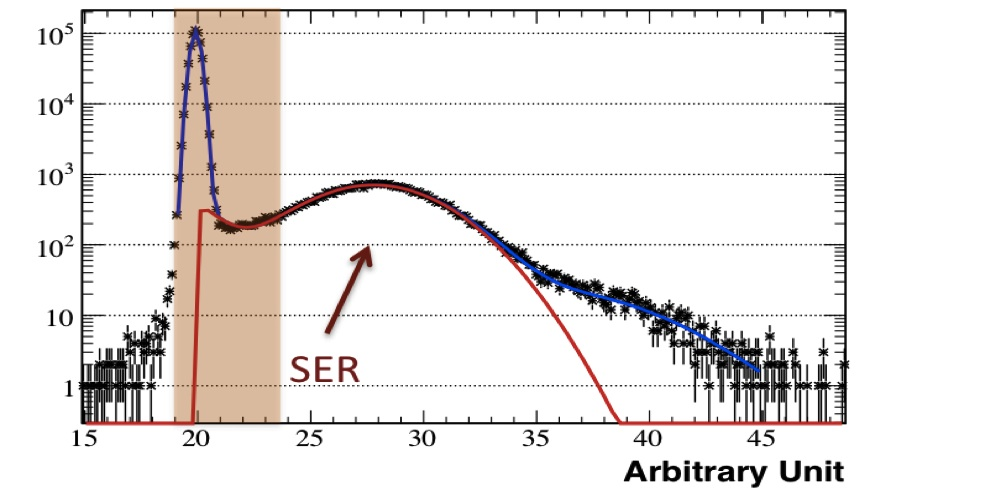
\includegraphics[width=\textwidth]{DC_Results/Gaussian_SER.jpg}
\label {Gaussian SER}
\end{figure}

In this graph, the highlighted region consists of the pedestal, which is the signal given by the PMTs which see no light, and the low energy part of the SER. Using the standard analysis tools, signals in the highlighted region are thrown away. Most of these signals, specifically the ones in the pedestal and in the ``dip" region are noise. However, you can see that there is a small fraction of SER events which are thrown away by the standard set of cuts. Potentially, one could save those low amplitude signals by making use of a different set of cuts, but at the risk of  contaminating the signals with low-amplitude noise from the pedestal and the ``dip" region.

To test if it's possible to capture these low charge channels without increasing the amount of noise, we developed an alternate analysis tool, with adjustable cuts as well as a "dummy integrator," a tool which has no noise rejection and just naively sums the charge over the entirety of a pulse. These tools are used after the pulse reconstruction step of data analysis, and produce per-channel charge calculations. Figure \ref{DI vs. SAT} compares the per-channel charge response of the ``dummy integrator" to that of the standard Double Chooz analysis tool. The channels with negative charge are expected as a result of a naive baseline subtraction on channels which see no signal. 

\begin{figure}
\caption{Dummy integrator compared to the standard analysis tool on Ge 68 Monte Carlo data.}
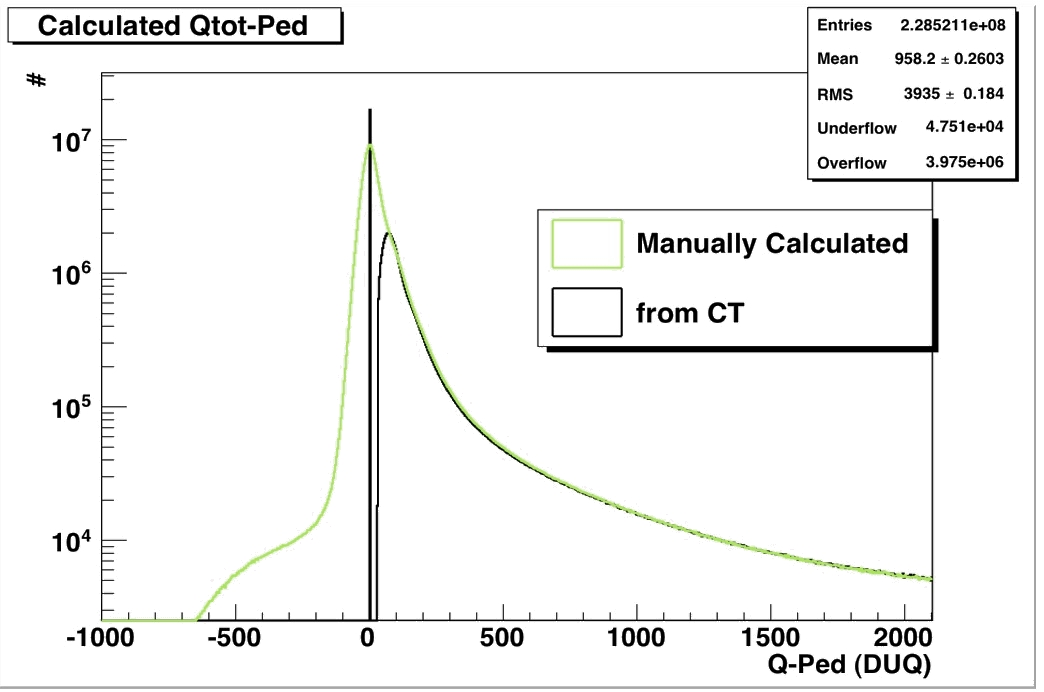
\includegraphics[width=\textwidth]{DC_Results/DI_Ge68_Colorized.jpg}
\label{DI vs. SAT}
\end{figure}

It can be seen that there is a region in which the manual tool captures charges that are discarded by the standard (Common Trunk, or CT) analysis tool. This is due to a pair of cuts that the CT tool puts on incoming signals: a total charge requirement and a current minimum requirement. The total charge requirement keeps pulses with total charge $Q_{pulse} > 5 \times RMS_{Ped} \times \sqrt{N_{bins}}$, where $RMS_{Ped}$ is the root mean square of the pedestal of the signal, with the pedestal being determined by the 10 nanoseconds of data before the start of the pulse, while $N_{bins}$ is the number of bins in the pulse time window and $ Q_{pulse}$ is in arbitrary units, referred to internally as DUQ (Digital Units of Charge) which are later calibrated into energy through the use of calibration systems and the known energy of the gadolinium capture peak. The raw pulse data is current as a function of time, in two nanosecond bins, for a total of 256 nanoseconds from the start of the pulse. 

The second requirement is that there be at least one bin in the pulse which has a current over 2 units (as above, these are arbitrary units which are later turned into physical units through calibration). Once the charge- and current-based requirements are applied to ensure that the pulse is not just a background fluctuation, the pulse start time is calculated by scanning over the bins and finding the first bin in which the current  is greater than 30\% of the maximal current. A diagram of this standard way of handling pulses can be seen in Fig. \ref{Standard Reco Pulse}.

\begin{figure}
\caption{Standard pulse reconstruction tool selecting the region between the two black dotted lines.}
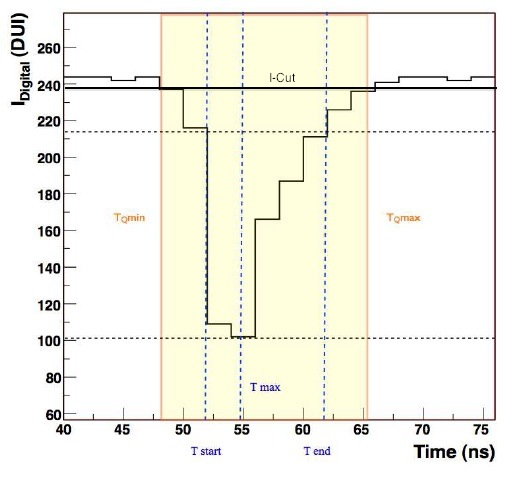
\includegraphics[width=\textwidth]{DC_Results/Standard_Reco_Pulse.jpg}
\label{Standard Reco Pulse}
\end{figure}


In the alternate analysis tool, the following changes are made. First, the charge-based cut was eliminated, though the current-based cut was kept. This was implemented to allow for more low-charge pulses to be kept. Second, the charge integration period was changed to begin 10 ns before the ``pulse start time." This includes more of the pulse, as beginning integration at the ``pulse start time" is guaranteed to miss some charge in the early bins. The pedestal subtraction was proportionally increased by the expansion of the integration window, so the danger of adding additional pedestal charge was minimized. 

After these changes were implemented, the CT Reco Pulse and our alternate analysis tool were tested against each other to see which tool induced the largest error in reconstruction. Additionally, a third algorithm, which integrates over the full 256 ns of pulse with no cuts, was used as a sanity check. This test was performed by generating a set of MC data corresponding to four different isotopes in the center of the detector: $^{137}Cs$, $^{68}Ge$, $^{60}Co$, and $^{252}Cf$. The three reconstruction algorithms were then used on the four data sets, producing an ``energy response" function for them. This energy response is scaled such that all of the algorithms reconstruct the 2.2 MeV hydrogen (n,$\gamma$) capture of $^{252}Cf$ neutrons at the proper value. The scaled energy responses of the three algorithms are then checked at four points, and their deviations are compared to the true energy. A plot of the results can be seen in Fig. \ref{Three Tool Comparison}. 

\begin{figure}
\caption{Three tool comparison, showing the superior performance of the alternate tool at lower energies.}
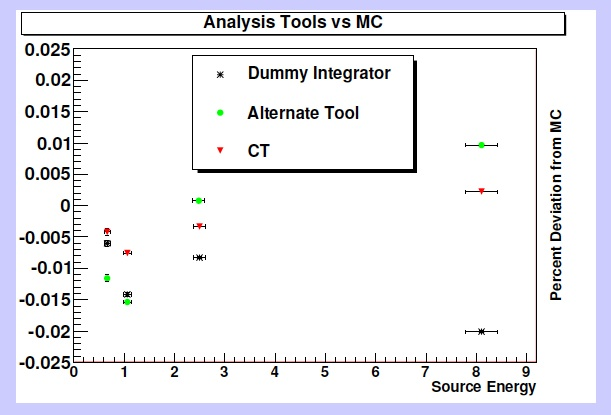
\includegraphics[width=\textwidth]{DC_Results/Ana_Tool_Comp}
\label{Three Tool Comparison}
\end{figure}


As can be seen, the alternate analysis tool performs better than the standard tool close to the 2.2 MeV peak, but at higher energies the standard analysis tool is superior. The delayed part of the neutrino signal is at the 8 MeV capture peak. In this region the standard analysis tool performs a more accurate energy reconstruction. Therefore, the alternate analysis tool was not used as a part of official Double Chooz publications, but remains a useful tool for examining changes to the energy scale in the very low energy region.   

\subsection{PMT Gain Calibration}
\label{sec:PMT_Calibration}
As photomultiplier tubes (PMTs) are the primary detection devices used by Double Chooz, understanding their behavior is vital for the experiment. The signal produced by a PMT in response to an incoming photon must be known for the proper determination of $\theta_{13}$.  In general, the charge produced by a PMT is approximately linear to the energy of the incoming event, with the charge out being related to the charge in by $Q_{Out}= G^{\prime} \cdot Q_{In}$. Since the experiment uses Analog to Digital Converters to map charge to a digital value, we can include them in the signal chain calculation by expressing signal not in terms of  charge, $Q_{Out}$, but in terms of ``ADC" counts, {\it A}. 

This change of variables to those which are directly measured by the experiment gives the following expression: $A = G \cdot Q_{In} + A_{P}$, where $A_{P}$ is the pedestal of the ADC, and $G$ is the gain. The pedestal is the ADC value when there is no signal, and is typically well-described by a Gaussian with a mean and variance of $\mu_{p}$ and $\sigma_{p} $ respectively. With this basic picture established, we now add some additional complexity in the description of the response of the PMTs to incoming photons. 

PMTs produce a discrete number of photoelectrons at the photocathode when struck by a light signal, but one photon can produce at most one photoelectron. The response to a single photoelectron is well described by two possible profiles: Gaussian and exponential. For an exponential-response PMT $P_1(Q)$, the probability that a single photoelectron signal produces an output charge {\it Q} is $P_1(Q) = \frac{1}{q_0}e^{-\frac{Q}{q_0}} \Theta(Q)dQ$ with $\Theta$ being the Heavyside step function. For a Gaussian response, $P_1(Q) = \frac{1}{\sigma \sqrt(2\pi)}e^{-\frac{-(Q-q_0)^2}{2(\sigma^2)}} \Theta(Q)dQ$.

From these distributions, it's possible to extract the mean, $\mu$ and variance, $\sigma^2$. For the Gaussian case, $\mu_g = q_0$ and $\sigma_g^2 = \sigma^2$, while for the exponential case,   $\mu_e = q_0$ and $\sigma^2_e = 2q_0^2$.  For most signals the PMT detects more than one photoelectron. In fact, the number of photons, {\it n}, seen by a PMT in response to a  light signal of some arbitrary fixed strength is well described by a Poisson distribution, $P(n;\mu) = \frac{\mu}{n!}e^{\mu}$,  where $\mu$ is the mean value of the distribution. A particular feature of the Poisson distribution is the relation between the mean, E, and the variance, $V$:  $E[n, P(n; \mu)] = V[n, P(n;\mu)] = \mu$. 

Since we know the response of a PMT to a single photon signal, the response of a PMT to a set of constant-energy light pulses with Poisson mean $\mu$ can be determined. The response of a PMT to a single photon is $P_1(Q)$, and, therefore, the response of the PMT to {\it N} photons is obtained by convolving the single event distribution with itself  {\it N} times. We shall proceed assuming an exponential probability distribution for the single photoelectron response, $P_1(Q)$. These results are easy to replicate for the case of a Gaussian response, and the results of this analysis for a Gaussian PMT will be given at the end of the chain of calculation.  


It can be readily determined that the result of N convolutions of $P_1(Q)$ with itself, $P_N(Q)$,  is $P_N(Q) = \frac{Q^{N-1}}{(N-1)!q_0^N}e^{-Q/q_0}$. The distribution has a mean value of $\mu=nq_0$ and a variance $\sigma^2=n(n+1)q_0^2$. We don't know the exact number of photons that will be arriving, but the number of photoelectrons that will be produced is defined by the Poisson distribution, $P(n;\mu)$. Therefore, the expected signal that will be arriving is described by a probability distribution $P_\mu(Q) = \sum \limits_0^\infty P(N, \mu)P_{N}(Q)$. This sum can be expressed analytically as $P(Q; \mu) = \frac{1}{q_0}\sqrt{\frac{\mu q_0}{Q}}I_1(2\sqrt{\frac{\mu Q}{q_0}})e^{-(\mu+Q/q_0)}$ with $I_1$ being the modified Bessel function of the first order. A comparison of this analytic probability distribution to a simplified MC model can be seen in Fig. \ref{PMT_Cal_MC}:.

\begin{figure}
\caption{Analytic charge probability distribution compared to Monte Carlo for $\mu =0$ and $q_0=1$, showing strong agreement \cite{PMTCalibration}.}
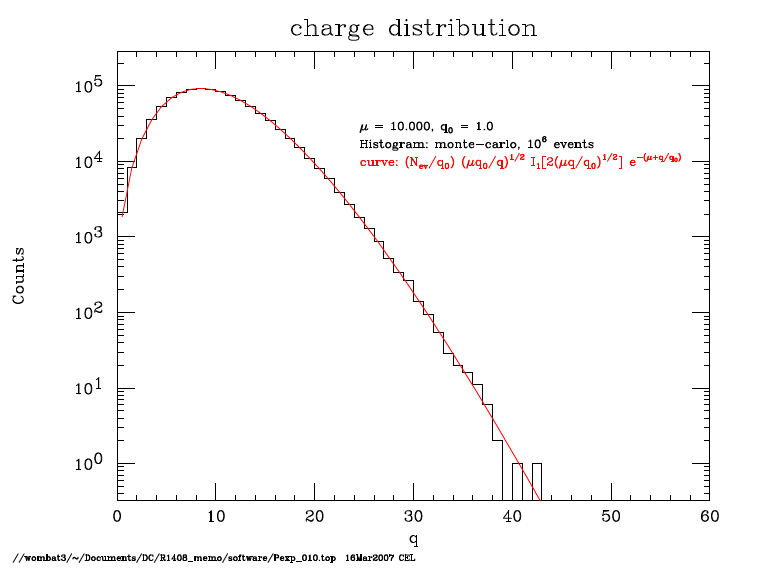
\includegraphics[width=\textwidth]{DC_Results/PMT_Cal_MC_Comp.jpg}
\label{PMT_Cal_MC}
\end{figure}

With the analytic expression validated, one can use it to calculate the expectation value and variance of a PMT that sees a light signal as described above. Specifically, $\mu_{expectation} = q_0 \mu_{Poisson}$ and $\sigma^2 = 2 q_0^2 \mu$. These results are validated against a Monte Carlo model in Fig. \ref{photostats_MC}. 


\begin{figure}
\caption{Comparison of calculated statistical values to Monte Carlo, showing strong agreement \cite{PMTCalibration}.}
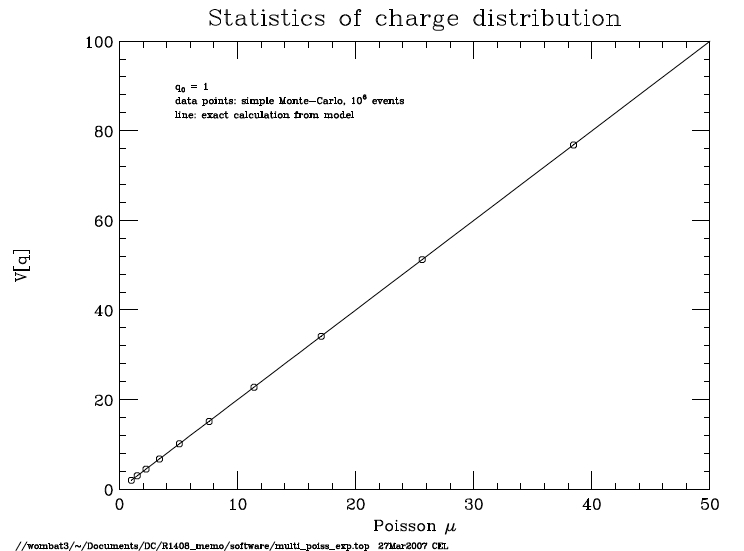
\includegraphics[width=\textwidth]{DC_Results/Photostats.jpg}
\label{photostats_MC}
\end{figure}

As noted previously, this same procedure can be performed with a Gaussian single photoelectron response, as well as for an exponential. The point of divergence for this sort of PMT arises with the self-convolution of the Gaussian response function. Making use of the Fourier transform property that maps convolution to multiplication in wavelength space, we can arrive an an analytic expression for the convolution of a Gaussian by itself n times, $P^{Gaussian}_n{Q}$. Specifically, $P^{Gaussian}_n(Q) = a e^{\frac{-(x-b_n)^2}{2c_n^2}}$ where $c_n = \sqrt{nc_1^2}$ and $b_n$ = $nq_0$. This is another Gaussian with a mean which is the sum of the means of the original Gaussian and a variance which is the quadratic sum of the variances.  The rest of the calculation follows as above, but with the substitution of the Gaussian form for the exponential one. 

To add an additional wrinkle into our analysis is the fact that we digitize charge by running it through an ADC. The value that is then returned depends not only on the gain of the ADC, but also on the mean and variance of the pedestal of the ADC, as noted previously. Using the statistical values calculated previously, $A_{exp} = G \mu q_0 + \mu_p$, where $A_{exp}$ is the expected ADC  value and $\mu_p$ is the mean value of the pedestal, and $\sigma^2_{exp}= G^2 2\mu q_0^2 + \sigma_p^2$, with  $\sigma^2_p$ being the variance of the pedestal.  

Our desire is to isolate the gain (in ADC counts per photoelectron) {\it G} from the calculation above. Obviously, if there is no pedestal, taking the ratio of the two quantities gives $2Gq_0$, with $q_0$ being the mean charge detected for a single photoelectron. However, since real ADCs have a pedestal, this simple ratio doesn't work. Instead, if one varies $\mu$ by varying the level of the light signal, the contribution of the pedestal is constant. Therefore, if one varies the light level, the effects of the pedestal will not change, allowing one to isolate the gain by taking data from a PMT at a variety of different light levels, then plotting variance against mean, and taking the slope of the resulting line. 

Another way of determining gain is to measure the ADC values resulting from a pulse generated by a single photoelectron. If the measured pulse is produced by one and only one photoelectron, the gain, will be given by $G= A/q_0$, since one does not have the pedestal contribution if pedestal pulses are able to be excluded. One can exclude the pedestal by implementing a threshold value of charge such that the pedestal falls below the threshold. This single photoelectron peak method of gain calibration is much faster than the use of photostatistics, since the photostatistics method relies on having large amounts of data at multiple energies, but the single photoelectron peak method relies on having a light pulse of sufficiently small intensity such that the PMT being calibrated produces a single photoelectron response, something that requires additional apparatus for most commercial LEDs. 

To confirm that the two methods give equivalent gains for the exact same PMT, we built a test apparatus at Drexel University and tested two different PMTs, a Hammamatsu R1408 PMT  and a Hammamatsu R7081 PMT. These two PMTs were chosen because they are the PMTs that are used in the IV and Buffer of Double Chooz, respectively. To reduce noise and the risk of light leaks, the two PMTs were tested in copper-foil covered dark boxes. At the top of the dark box is mounted an LED, which is covered by a diffusion-filtered, black-painted can during the single photoelectron portion of the test. A diagram of the electronics used as a part of the setup can be seen in Fig. \ref{PMT Test Setup}.

\begin{figure}
\caption{PMT gain testing electronics block diagram.}
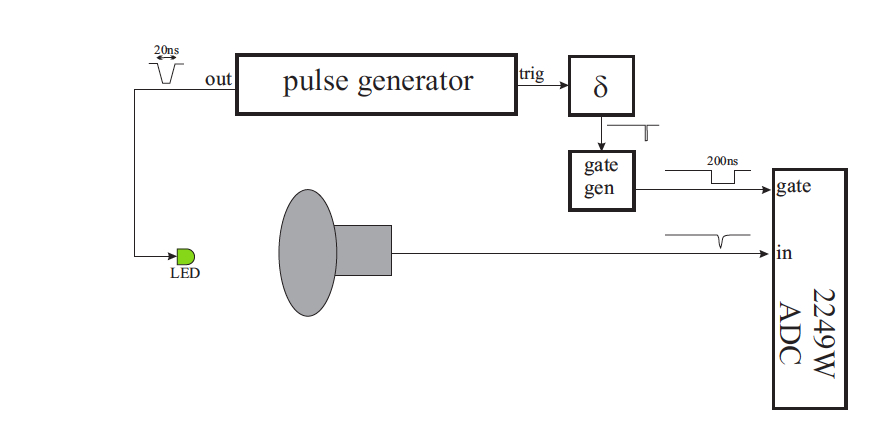
\includegraphics[width=\textwidth]{DC_Results/PMT_Electronics.jpg}
\label{PMT Test Setup}
\end{figure}


The gate system is required to ensure that the calibration signals that are being used are not contaminated by dark noise and to avoid problems associated with saturating the ADC. Since a gate system is required, delay must be put on the gate signal to ensure that the signal produced by the LED pulse falls entirely within the gated region of the ADC. For the photostatistics test we varied the amplitude of the pulse produced by the pulse generator causing the LED to produce differing levels of light. Because of the power of the photostatstics method, the exact relationship between pulse amplitude and light produced is not important, as the only requirement for the method to work is that the light pulses produce different numbers of photoelectrons. We applied pulses of 40 ns at various voltage levels, between 1 and 8 volts to the LED, and took 10,000 points per voltage. The means and standard deviations of the ADC readings at a given voltage were plotted against each other. The plot can be seen in Fig. \ref{Photostats 6416}.

\begin{figure}
\caption{Photostats mean and variance for PMT \#6416, showing linear fit up to saturation.}
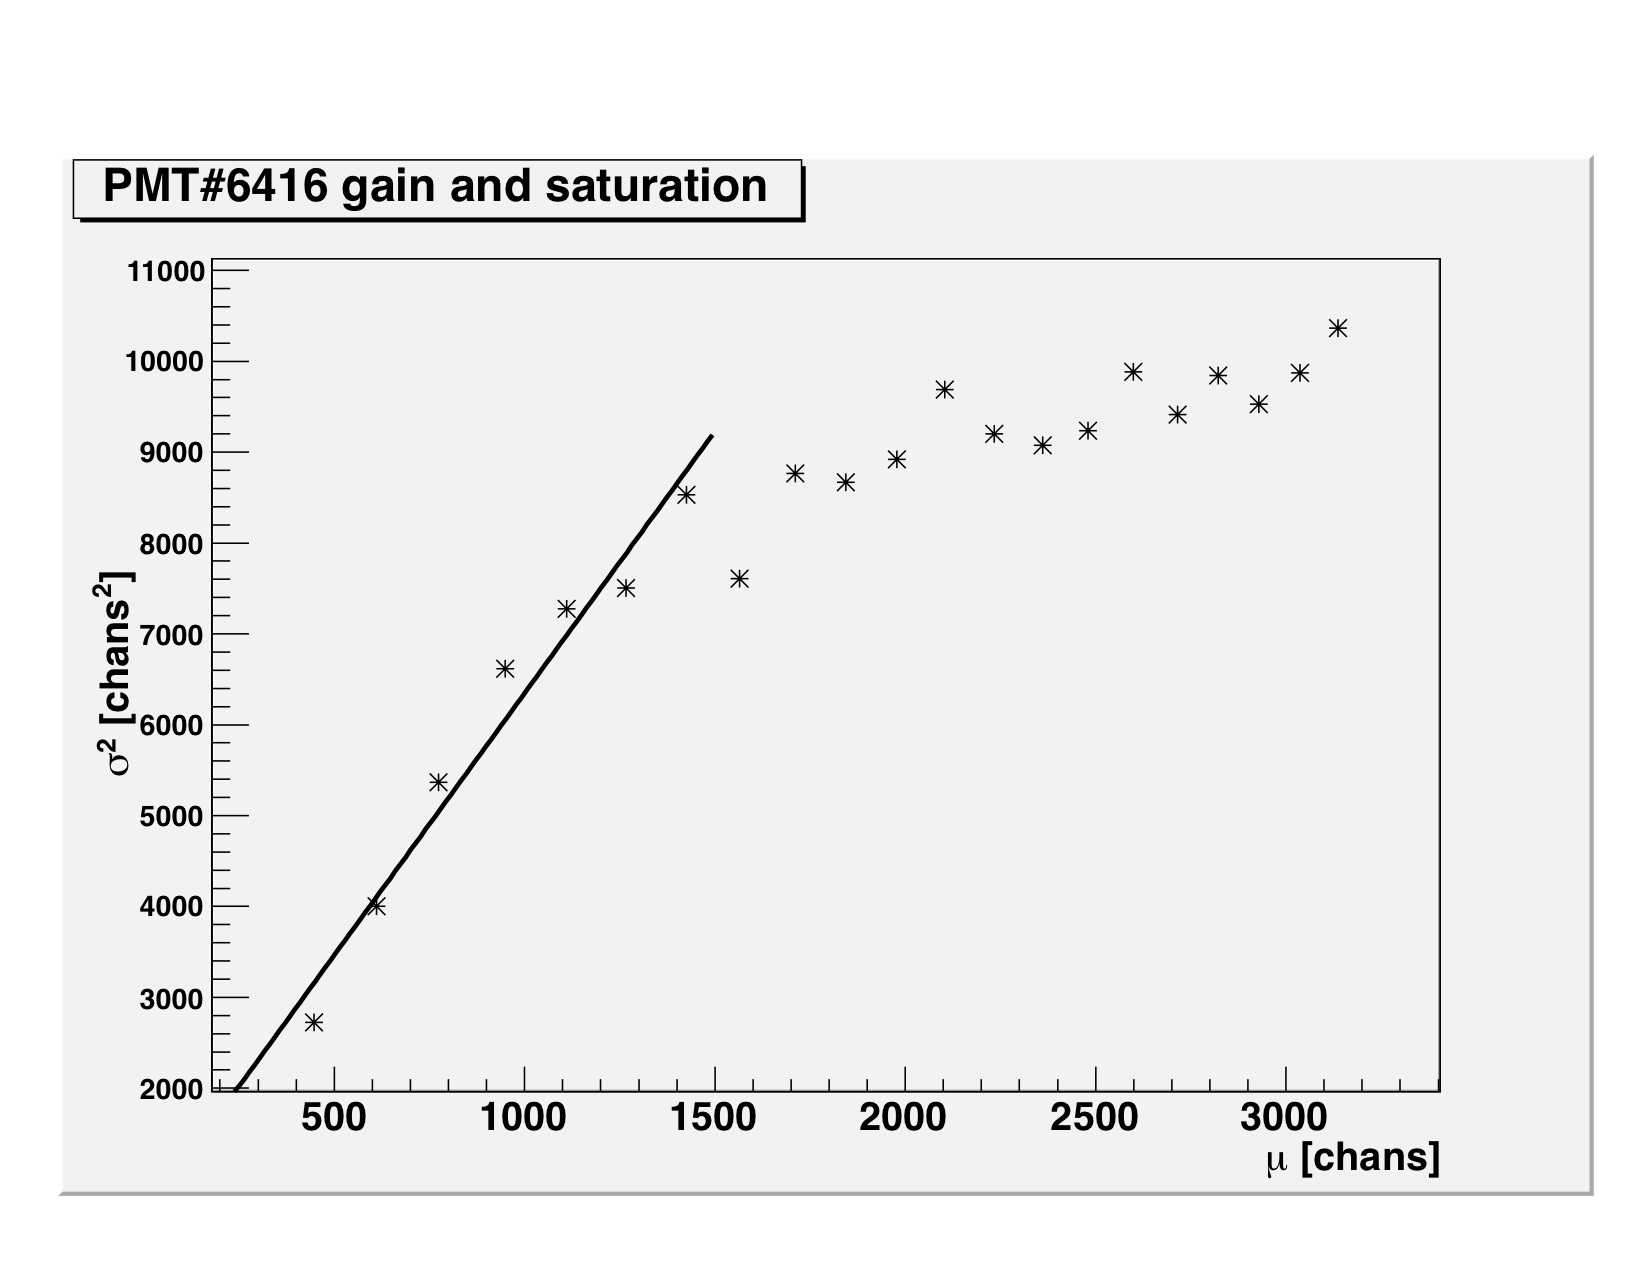
\includegraphics[width=\textwidth]{DC_Results/Photostats_Gain_6416.jpg}
\label{Photostats 6416}
\end{figure}

There are two regions in the plot in figure \ref{Photostats 6416}. The first region, which is fit by a line, is the useful signal region. Beyond $\mu = 1500$, the system saturates, meaning that increasing the signal does not increase the variance, following the relationship discussed above. Saturation is due to the ADC system used as part of the test, and is not a feature of expected Double Chooz signals.  Therefore, to extract the gain, one must consider only the first region and not the second. 

For the single phototelectron test, the pulse was reduced until the point that approximately half of the signals produced zero photoelectrons. Specifically, we fed pulses to 4.5 V of 20 ns in duration to the LED, and adjusted the high voltage being supplied to the PMT in 50 V steps.  The gain was then determined at each high voltage setting by fitting the histogram of ADC values with three functions, a Gaussian for the pedestal, an exponential for the gap between the pedestal and the single photoelectron peak in the data, and a Gaussian for the SPE peak. The mean of the Gaussian fit for the single photoelectron peak divided by $q_0$, the elementary charge unit, gives the gain. An example of the fitting technique used can be seen in Fig \ref{SPE Fit}.

\begin{figure}
\caption{Sample three-part fit of PMT \# 6416.}
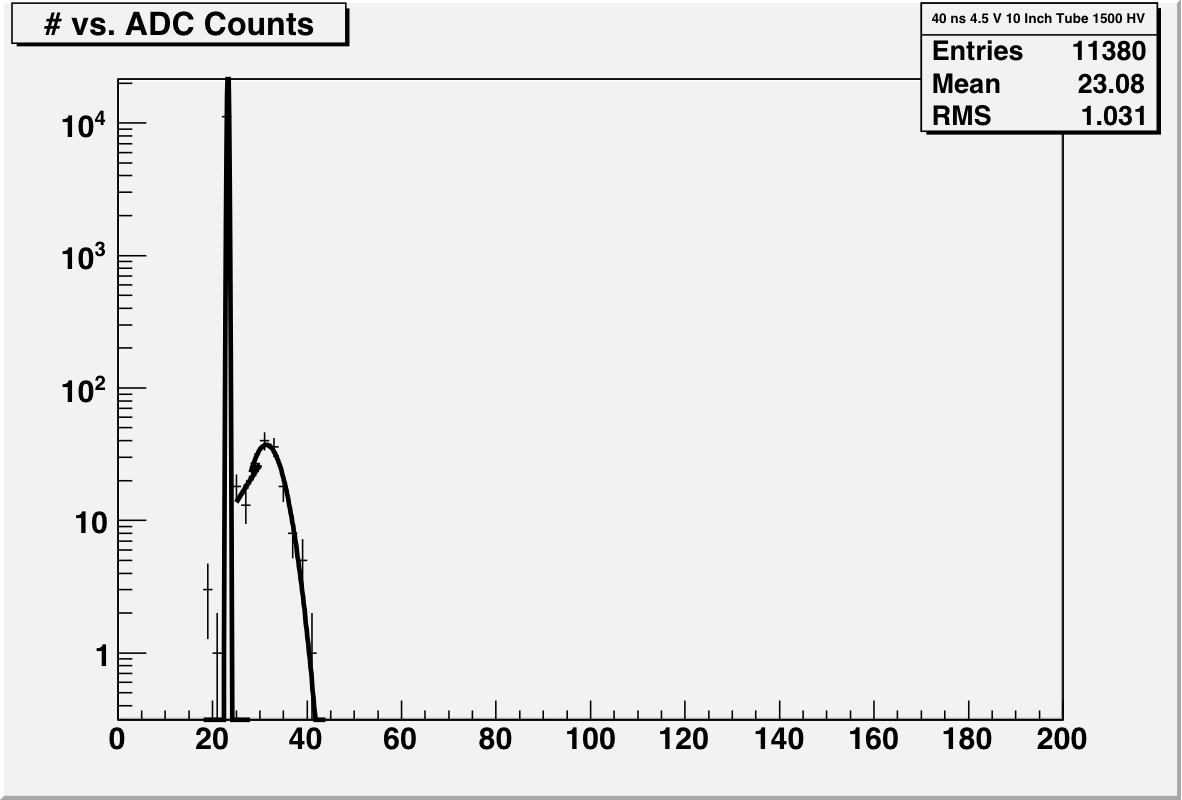
\includegraphics[width=.5 \textwidth]{DC_Results/SPE_Fit.jpg}
\label{SPE Fit}
\end{figure}

We compared the calculated gain using the two different methods with the PMT subject to 1500 V of high voltage. We found a gain value of $1.76 \times10^7 \pm 2.5 \times10^6$ using the photostatistics method and a gain of $1.58\times10^7 \pm1.3 \times10^6$ using the single photoelectron peak method. These two values are within 1 $\sigma$ of each other, implying that the two gain calibration methods are equivalent. This shows that the photostatistical gain calibration method is a useful addition to the set of calibration tools available to the Double Chooz collaboration. This tool is particularly useful for the inner veto PMTs, as they lack a well-defined single photoelectron peak, making the use of the photostatistics the best method for gain calibration. 

\section{Backgrounds}
\label{sec:Backgrounds}
Backgrounds to the Double Chooz experimental signal come in two forms, correlated and uncorrelated. Correlated backgrounds are those that mimic the prompt/delayed structure of the neutrino signal while uncorrelated backgrounds, or ``singles" have no such structure, but can by random chance combine to simulate a signal. The most dangerous of these background signals are the correlated backgrounds, which are most likely to mimic a neutrino signal. Nevertheless, singles can also masquerade as neutrino signals due to random coincidence.

Most correlated events are ultimately caused by cosmic-ray muons passing through or near the detector. Therefore, there are a number of measures in place to reduce the cosmic-ray muon background and to tag what muon events remain. The first layer of defense against cosmic ray muons is the location of the detector system, which has a substantial amount of rock overburden. The next layers of protection are the veto systems, inner and outer. 

The Outer Veto (OV) consists of a series of rectangular strips consisting of scintillating material with a wavelength shifting fiber in the center. These strips are arranged into rectangular modules, with a well-defined orientation, with the fibers terminating in a PMT. By layering the modules in perpendicular orientations, it's possible to isolate the position and direction of a muon traveling through Outer Veto. A diagram of the Outer Veto can be seen in Fig. \ref{OV}

\begin{figure}
\caption{Outer Veto system as it is deployed in the far detector.}
\centering
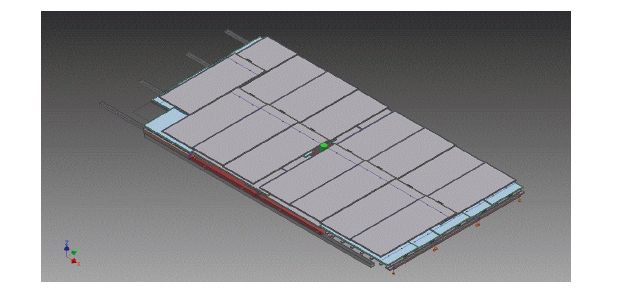
\includegraphics[width=\textwidth]{DC_Results/Outer_Veto.jpg}
\label{OV}
\end{figure}


The IV is filled with non-Gd-doped liquid scintillator and instrumented with 78 PMTs, in an arrangement optimized for detecting incoming cosmic ray muons: more upward-looking coverage than downward looking-coverage.  The Inner Veto is connected to the front end, and makes use of the same DAQ system. 

The two veto systems are designed to detect incoming muons and veto triggers from the NT for 1 millisecond after detection of a muon signal. Muon triggers are those that hit more than one strip in the OV, deposit more than 5 MeV in the IV, or more than 30 MeV in the Inner Detector. Vetoing in this matter reduces the correlated background enormously. 

For uncorrelated backgrounds there are three primary contributors, natural radioactivity in the detector and surrounding rock, PMT dark noise, and so-called ``light noise." Steps have been taken to mitigate these sources. In the case of natural radioactivity, strong radiopurity requirements were made and enforced for the most radioactive elements of the detector: the glass used in the PMTs.

Since PMTs are sensitive to single photons they have a certain number of signals even in absence of actual photons. These are dark rate events and tend to be single-photoelectron-level signals from a single PMT. However, since the dark rate of the Double Chooz PMTs is approximately 2 kHz, additional steps need to be taken to ensure that the dark rates do not pollute the neutrino data sample. Therefore, the charge reconstruction algorithm throws out signals with a maximal charge of $<$ 2 ADC counts, as well as signals which have a small total charge. 

The final source of uncorrelated background, light noise, was the least expected. The bases of the PMTs give off small electrical signals at random intervals which can be detected by PMTs. These events deposit energy primarily on the PMT from which the spark originates, with small energy depositions on other PMTs. 
	
The light noise is able to be filtered by implementing a cut based on comparing the amount of charge seen in a single PMT against the total charge seen by all PMTs, referred to as an MQTQ (Max Q over Total Q) cut. The fact that the light tends to be concentrated in a small number of PMTs also means that the pulse start times vary widely in a light noise event in comparison to a neutrino signal. Therefore, we make use of a dual cut in the RMS of the pulse start time and the MQTQ value of an event to strongly reject light noise. 

\section{Simulation}
  In addition to the powerful hardware tools developed for Double Chooz, there exists a suite of software tools to process, simulate, and analyze data from the experiment. Simulation of Double Chooz anti-neutrino flux is done through two main tools, DRAGON and MURE \cite{DC_2013}, the reactor simulation programs, and DCGLG4-sim, a GEANT4-derived particle/detector simulation environment. GEANT4 is the standard particle Monte-Carlo simulation program, used for applications ranging from proton therapy to the LHC \cite{G4}. 
  
\subsection{Reactor Simulation}
Simulation of the reactors is vital to the one-detector phase of the experiment, as knowledge of the reactor spectrum and the normalization of the neutrino flux are needed to determine the mixing angle $\theta_{13}$. To this end, two simulations environments for reactor burn-up were developed: MURE, which is a 3-D full reactor simulation making use of Monte Carlo neutron transport calculations and DRAGON, which is a 2-D simulation of the various fuel rod elements. 

The results of both of these codes are checked against a Takahama-3 reactor and were found to be in agreement with other similar simulations. The fuel in the reactor cores is replaced completely over the course of three years, with one third of the load being replaced every year. Fuel rods have enrichment rates ranging from 1.8\% to 4\%. Once the base information about the properties of the reactors is established the simulations proceed during the burn-up and are then cross-checked, giving the experiment its quoted uncertainty in its fission rate fractions.

\subsection{Detector Simulation}
Simulations of detector performance and response are handled at the lowest level by DCGLG4-sim (Double Chooz Generic-Land Geant-4) \cite{DCGLG4sim}. Adapted from simulations used with the KamLAND experiment, DCGLG4-sim has a number of powerful features that allow for very accurate simulations of the Double Chooz Experiment. These features include thermal neutron libraries accurate down to 4 keV, detailed simulation of the scintillator, including detailed light waveforms, spectra, re-emission, and Birks quenching. Positioning of the PMTs and detector geometry has been verified for use in the Monte Carlo through a photographic survey. 

The optical model has been heavily vetted by the collaboration, making use of the Compton scattering to calibrate the relative light yield of the NT and the GC. Further calibration of the simulation was performed through the deployment of calibration sources, which are detailed in the subsequent section. Additional tuning of the optical parameters of the simulations  was performed by measurements of the parameters of the scintillator in a lab environment.

The raw output of DCGLG4 is then run through ROSS (Read-Out-System-Simulation) to simulate PMT and electronic effects, allowing for a direct comparison of Monte Carlo and data. Monte Carlo and data can be mixed to allow for validation of cut efficiency and discrimination ability, if required. The data, mixed or unmixed, can then be run through the analysis Common Trunk, providing pulse and position reconstruction through RecoPulse and the various position reconstruction suites, such as RecoBAMA. 

\subsection{Signal Reconstruction}
\label{sec:RECO}
RecoBAMA is the primary tool used by the collaboration to determine the position of events inside of the detector. It makes use of a dual technique to fit the position of point-like events, incorporating both time and charge-based fitting of events. Time-based fitting relies on knowing the index of refraction of the liquids inside of the detector. Assuming an event occurs at a time $t_0$, the light will have travelled a distance $d= \Sigma(t-t_o) \cdot c_n$, where $c_n$ is the speed of light in each of the three media: Gd-doped target scintillator, undoped gamma-catcher scintillator, and the mineral oil in the buffer. Working backward, the algorithm grows spheres from the signal-seeing PMTs of radius $r =\Sigma (t_i-t_0) \cdot c_n$, where $t_i$ is the time at which the PMT i saw a signal. Where the spheres intersect is the position at which the event occurred. 

Meanwhile, the charge-based reconstruction works on a similar principle. The photons produced by an event inside the detector are absorbed and re-emitted via scintillation, producing a ``sphere" of light. Naturally, the intensity of the light falls off as $\frac{1}{r^2}$ to first order, but there are additional considerations that must be taken into account. Using both charge- and time-based reconstruction allows for much fuller picture of the nature of events than either alone. 

\section{Results}
At present, the Double Chooz experiment is still in the one-detector phase of operation but, despite this, has far exceeded the power of Chooz, providing nearly 3-$\sigma$ determination of the value of $\theta_{13}$.  This analysis is, as noted in prior sections, based upon a search for a two-fold coincidence of a prompt positron annihilation followed by a delayed neutron capture on gadolinium (an ``IBD" event). To identify IBD events, many cuts needed to be applied.  First, we require that the prompt and delayed events fall within 2 and 100 $\mu$s of each other. These cuts are informed by the 30 $\mu$s capture time of neutrons on Gadolinium. 

 To reduce muon-induced backgrounds, we rejected all events that occur within 1 ms after a cosmic-ray muon is detected within the IV or the ID. Next, we applied a ``light noise" cut,  as discussed in Sec. \ref{sec:Backgrounds}. We then applied a set of coincident selection cuts to the remaining events. Prompt (positron-like) events with energy between 0.7 MeV and 12.2 MeV were kept, and all others were discarded.  Delayed (Gd- Capture like) events with energy between 6.0 MeV and 12.0 MeV were kept, while all others were discarded. Finally, we impose a multiplicity cut, requiring that all there are no triggers within the 400 $\mu$s after a prompt event, other than a single delayed trigger. Moreover, we only keep prompt events which have no event within the 100 $\mu$s prior to the event.  This gives a sample of 8440 events that follow a Gadolinium-like selection. 
 
 To determine the efficiency of the cuts, the neutrino candidates are compared to high-statistics Monte Carlo signal and to calibration data. The table in Fig. \ref{Cut_Summary} summarizes the calculated efficiency of the cuts. 
 
 \begin{figure}
 \caption{Cut efficiencies on a per-cut basis for the Double Chooz result.}
 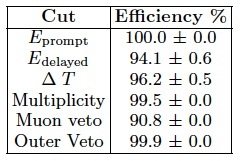
\includegraphics[width =.5 \textwidth]{DC_Results/Cut_Summary.jpg}
 \label{Cut_Summary}
 \end{figure}
 
 
 \begin{figure}
 \caption{Prompt and delayed neutrino candidate energies showing the Gd and Positron annihilation peak.}
 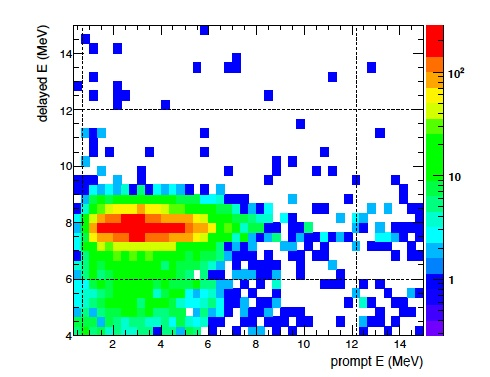
\includegraphics[width = .5 \textwidth] {DC_Results/Prompt_Delayed.jpg}
 \label{PromptDelay}
 \end{figure}
 
 \begin{figure}
 \caption{Time delay between prompt and delayed triggers, informing the use of the time cuts.}
 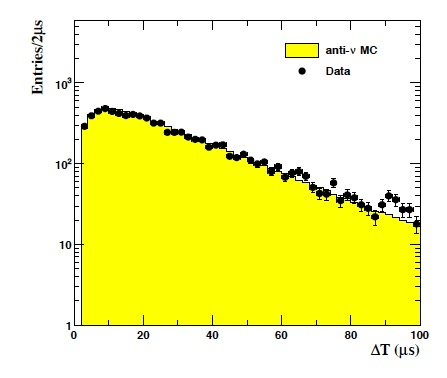
\includegraphics[width = .5 \textwidth]{DC_Results/Time_Dist.jpg}
 \label{PD_Time_Dist}
 \end{figure}
 
We then continue the analysis by binning the neutrino candidate in a set of variable sized bins with energy between 0.7 and 12.2 MeV. To increase differentiation power, the data is separated into two different periods; one contains data from the time period in which one reactor is operating at less than 20\% of nominal thermal power (On/Off), while the other consists of all other time periods (On/On). 

The binned neutrino candidates are then compared to a predicted spectrum of signal and background, with the predicted spectrum being calculated independently for the On/On and On/Off time periods. A comparison of the predicted neutrino events in each period compared to the actual number of candidates can be seen in \ref{IBD_Summary}. 

\begin{figure}
\caption{Neutrino candidates and backgrounds in the two periods, On/On and Off/Off.}
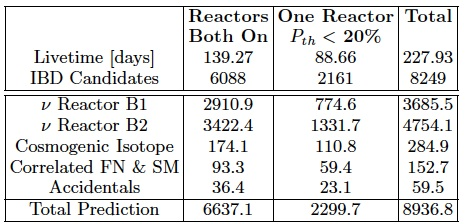
\includegraphics[width=.5 \textwidth]{DC_Results/IBD_Summary.jpg}
\label{IBD_Summary}
\end{figure}


The neutrino candidates were then fit to a two-neutrino oscillation hypothesis by $\chi ^2$ minimization where $\chi^2$ is given by Eqn. \ref{eq:X^2}. 
\begin{multline}
 \chi^2 = \sum^{36}_{i,j} (N_i - N_{i}^{pred} ) \times (M_{ij}^{Total})^{-1}(N_j - N_j^{pred})^{T} + \frac{(\epsilon_{FN/SN} -1)^2}{ \sigma^2_{FN/SM}} + \\
 \frac{(\epsilon_{9^Li} -1)^2}{\sigma^2_{^9Li}} + \frac{(\alpha_{E} -1)^2}{\sigma^2_{\alpha_{E}}} + \frac{(\Delta m^2_{31} - (\Delta m^2_{31})_{MINOS})^2}{\sigma^2_{MINOS}} 
 \label{eq::X^2}
 \end{multline}
 
 The fit parameters $\epsilon_{FN/SM}$ and $\epsilon_{^9Li}$ which scale the rates of the two backgrounds and are allowed to vary as part of the fit . The rate of accidentals is not allowed to vary as its uncertainty was precisely determined. The energy scale factor is allowed to vary linearly according to the $\alpha_{E}$ parameter with $\sigma_{\alpha_E} = 1.13\%$. $M^{Total}_{ij}$ is the total covariance matrix, which relates bin to bin uncertainties. The last parameter, $ \Delta m^2_{31}$, is the neutrino mass splitting, and is constrained by the MINOS \cite{MINOS} measurement of $\Delta m^2_{31} = (2.32 \pm 0.12) \times 10^{-3}$ . However, fitting without the MINOS constraint in the region  $\Delta m^2_{31} < 0.01 eV^2$ produces a $\Delta m^2_{31}$ value of $2.7 \pm 1.9 \times 10^-3 eV^2$, which is fully consistent with the MINOS result. The unrestricted-mass-splitting fit also gives a value of $\sin^2 (2 \theta_{13})$ which is consistent with the fit produced by including the MINOS constraints. 
 
 Uncertainties on the fit are handled through use of a set of covariance matrices $M^{x}_{ij}$. $M^{total}_{ij} =  M^{sig}_{ij} + M^{det}_{ij} + M^{stat}_{ij} + M^{eff}_{ij} + \sum_{b}^{back} M^{b}_{ij}$. The various separate independent covariance matrices represents the covariance between the predicted number of neutrino candidates in the spectral binning. Each element of each of the covariance matrix is recalculated as a function of the parameters used during minimization. Doing so allows for maintenance of the fractional systematic uncertainties, which would otherwise not be maintained due to the change of bin populations during the fit procedure. 
 
 The best fit yielded by this method is $\sin^2 2 \theta_{13} = 0.109 \pm 0.030$(stat.)$\pm 0.025$(syst.) with a  $\Delta m^2_{31}$ value of $2.32 \times 10^{-3} eV^2$ with $\chi^2/NDF = 42.1/35$.  This fit takes full advantage of the neutrino rate and spectral shape. A rate-only analysis yields a best fit of $\sin^2 2 \theta_{13} = 0.0170 \pm 0.052$ with $\chi^2/NDF = 0.50/1$, giving a probability of compatibility of 30\%. The results of this fit are displaced graphically in Fig. \ref{Best Fit}.
 
 \begin{figure}
 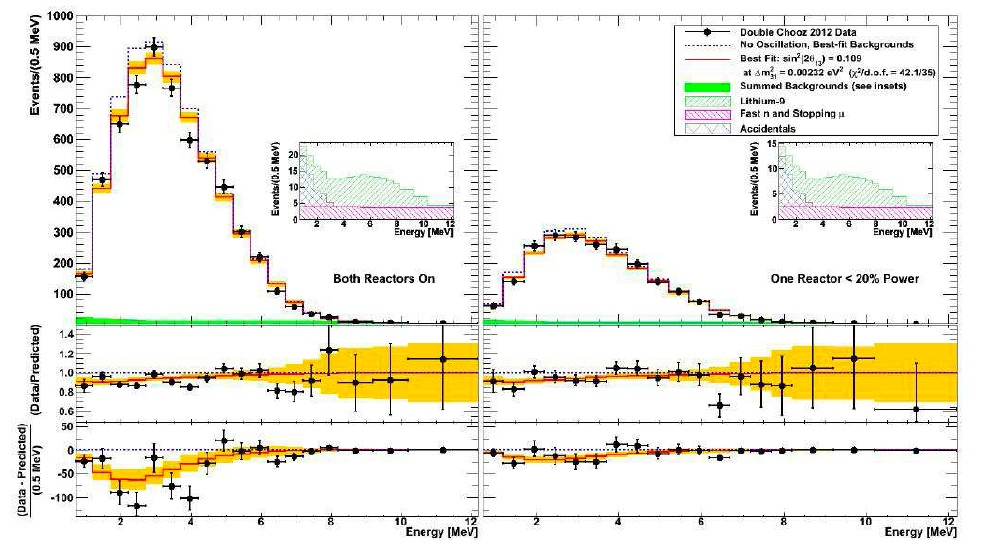
\includegraphics[width = \textwidth]{DC_Results/Best_Fit.jpg}
 \caption{Measured prompt energy spectrum for each integration period (data points) superimposed on the expected prompt
energy spectrum, including backgrounds (green region), for the no-oscillation (blue dotted curve) and best-fit (red solid curve)
at $\sin^2 2 \theta_{13} = 0.109$ and $\Delta m^2_{31}= 2.32 \times 10^{-3} eV^2$. Inset: stacked spectra of backgrounds. Bottom: differences between data
and no-oscillation prediction (data points), and differences between best fit prediction and no-oscillation prediction (red curve).
The orange band represents the systematic uncertainties on the best-fit prediction. \cite{DC_2012}.}
 \label{Best Fit}
 \end{figure}
 
Figure \ref{Fit Error} gives the uncertainties of the best fit parameters. The reactor flux uncertainty is the largest single factor, but will be completely eliminated once the near detector phase of Double Chooz begins, as the comparison between the neutrino flux at the two sites will be used without reference to the reactor flux. Improvements to the error caused by cosmogenic isotopes and the fast neutron/stopping muon (FN/SM) background have been the subject of a great deal of ongoing analysis, and a Double Chooz paper currently in production reduces these uncertainties a great deal. The next largest term, statistics, will be reduced both with time (there are about 50 neutrino candidates per day currently) and with the introduction of the near detector, which will more than double the expected neutrino rate due to doubling the existing sensitive volume at a closer location, and hence with a larger neutrino flux. 

The detector efficiency and detector response, however, are best improved through calibration. The ability to deploy calibration sources at off-axis points inside of the NT, particularly $^{252}$Cf will greatly help to reduce the error produced by the spill in/spill out effects, as well as to examine the Gd capture fraction throughout the volume. Additionally, the energy scale measurement would be much improved through the use of off-axis deployment of sources of various energies and particle types, as the response of the scintillator to electrons and gamma-rays varies. These considerations point to the use of a novel calibration system, able to deploy a variety of different sources at arbitrary points inside the detector. 

\begin{figure} 
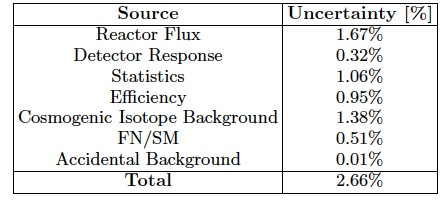
\includegraphics[width = .5 \textwidth]{DC_Results/Fit_Errors}
\caption{Contributions to the error on the $\sin^2 2 \theta_{13}$ analysis.}
\label{Fit Error}
\end{figure}
 